\chapter{Optimización convexa}\label{ChapterG} 
% chktex-file 8
% chktex-file 12
% chktex-file 13
% chktex-file 44

En muchos problemas de estimaciones estadísticas y regresión, la solución requiere el uso de métodos iterativos u optimización numérica. Aquí se verán los conceptos básicos de optimización convexa y se presentará el método de descenso de gradiente.

\section{Introducción}

\noindent Un problema de optimización matemática tiene la forma 
\begin{align}
\text{minimize } \quad & f_0(\mathbf{x}) \\
\text{subject to } \quad & f_i(\mathbf{x}) \leq 0, \quad i = 1, \ldots, m \\
& h_i(\mathbf{x}) = 0, \quad i = 1, \ldots, p 
\end{align}

\noindent donde el vector $\mathbf{x} = (x_1, \dots, x_d)^T \in \mathbb{R}^d$ es la variable de optimización, la función $f_0: \mathbb{R}^d \to \mathbb{R}$ es la función objetivo, las funciones $f_i: \mathbb{R}^d \to \mathbb{R}$, $i = 1, \dots, m$ son las restricciones de desigualdad y las funciones $h_i: \mathbb{R}^d \to \mathbb{R}$, $j = 1, \dots, p$ son las restricciones de igualdad. El dominio del problema es 
\begin{equation*}
\mathcal{D} = \text{dom}(f_0) \cap \text{dom}(f_1) \cap \cdots \cap \text{dom}(f_m) \cap \text{dom}(h_1) \cap \cdots \cap \text{dom}(h_p)
\end{equation*}

El conjunto factible o viable es el conjunto de puntos pertenecientes a $\mathcal{D}$ que satisfacen todas las condiciones o ligaduras (el conjunto de soluciones factibles). El conjunto óptimo es el conjunto de puntos factibles para los que la función objetivo alcanza su valor óptimo, denotado por $f^*$. Así, un punto $x^*$ es óptimo si pertenece al conjunto óptimo. 

\section{Optimización convexa}

\subsection{Conjuntos convexos}

\noindent Un conjunto $C \in \mathbb{R}^d$ es convexo si 
\begin{equation}
\theta x + (1 - \theta)y \in C, \quad \forall x, y \in C, \; \theta \in [0, 1]
\end{equation}
con $\theta \in \mathbb{R}$ forma un segmento de línea desde $x$ hasta $y$. Sean $x, y$ dos puntos en $\mathbb{R}^d$ tales que $x \neq y$. Los puntos de la forma 
\begin{equation}
z = \theta x + (1 - \theta)y, \quad \theta \in [0, 1]
\end{equation}

\noindent forman un segmento de línea que une $x$ con $y$. De forma más intuitiva, un conjunto convexo es aquel en el que el segmento que une dos puntos cualesquiera contenidos en ese conjunto, este también contenido en el conjunto (ver figura \ref{fig:conjuntoconvexo}).

\begin{figure}[h]
    \centering
    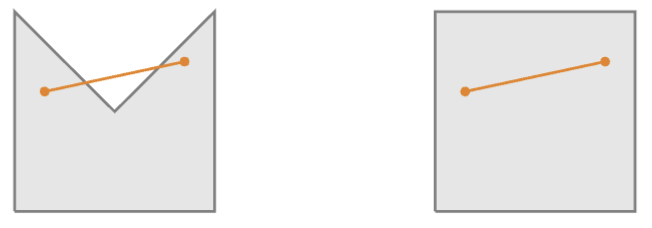
\includegraphics[width=0.6\textwidth]{fotos/65.png}
    \caption{A la izquierda un ejemplo de conjunto no convexo (ya que el segmento que une dos puntos de $C$ no está contenido totalmente en $C$) y a la derecha un ejemplo de conjunto convexo.}
    \label{fig:conjuntoconvexo}
\end{figure}

\subsection{Funciones convexas}

Una función $f: \mathbb{R}^d \to \mathbb{R}$ es convexa (figura \ref{fig:funcionconvexa}) si su dominio es un conjunto convexo y si para todo $x, y \in \text{dom}(f)$ y $\theta \in [0, 1]$ se cumple que
\begin{equation}
f(\theta x + (1 - \theta)y) \leq \theta f(x) + (1 - \theta)f(y)
\end{equation}

\begin{figure}[h]
    \centering
    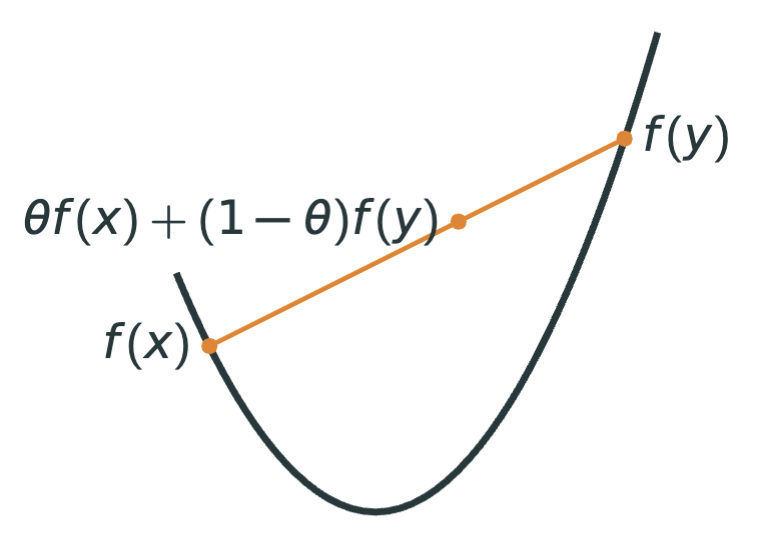
\includegraphics[width=0.4\textwidth]{fotos/66.png}
    \caption{A la izquierda un ejemplo de función no convexa y a la derecha un ejemplo de función convexa.}
    \label{fig:funcionconvexa}
\end{figure}

Una función $f: \mathbb{R}^d \to \mathbb{R}$ es estrictamente convexa si su dominio es un conjunto convexo y si para todo $x, y \in \text{dom}(f)$ con $x \neq y$ y $\theta \in (0, 1)$ se cumple que
\begin{equation}
f(\theta x + (1 - \theta)y) < \theta f(x) + (1 - \theta)f(y)
\end{equation}

Como ejemplos de funciones típicas convexas se tienen funciones afines, funciones cuadráticas, función de pérdida de mínimos cuadrados, \dots

\subsection{Caracterizaciones de primer y segundo orden}

Sea $f: \mathbb{R}^d \to \mathbb{R}$ una función diferenciable. El gradiente de $f$ en $x \in \mathbb{R}^d$ viene dado por 
\begin{equation}
\nabla f(x) = \left( \frac{\partial f(x)}{\partial x_1}, \dots, \frac{\partial f(x)}{\partial x_d} \right)^T
\end{equation}

\noindent donde el vector gradiente da la dirección de mayor cambio de $f$. Sea ahora $f: \mathbb{R}^d \to \mathbb{R}$ dos veces diferenciable. El Hessiano de $f$ en $x \in \mathbb{R}^d$ viene dado por
\begin{equation}
\nabla^2 f (x) = 
\begin{pmatrix}
\frac{\partial^2 f(x)}{\partial x_1^2} & \cdots & \frac{\partial^2 f(x)}{\partial x_1 \partial x_d} \\
\vdots & \ddots & \vdots \\
\frac{\partial^2 f(x)}{\partial x_d \partial x_1} & \cdots & \frac{\partial^2 f(x)}{\partial x_d^2}
\end{pmatrix}
\end{equation}

\noindent Las aproximaciones de Taylor a primer y segundo orden toman la forma 
\begin{gather}
f(y) \approx f(x) + \nabla f(x)^T(y - x) \\
f(y) \approx f(x) + \nabla f(x)^T(y - x) + \frac{1}{2}(y - x)^T\nabla^2 f(x)(y - x)
\end{gather}

\subsubsection{Caracterización de primer orden}
Sea $f: \mathbb{R}^d \to \mathbb{R}$ una función diferenciable. Entonces $f$ es convexa si y solo si su dominio es convexo y $\forall x, y \in \text{dom}(f)$
\begin{equation}
f(y) \geq f(x) + \nabla f(x)^T(y - x)
\end{equation}

Nótese que si $\nabla f = 0$, entonces $\forall y \in \text{dom}(f)$ se tiene que $f(y) \geq f(x)$, es decir, $x$ es un mínimo global de $f$. La aproximación de Taylor de primer orden es un subestimador global de $f$.

\subsubsection{Caracterización de segundo orden}
Sea $f: \mathbb{R}^d \to \mathbb{R}$ dos veces diferenciable. Entonces $f$ es convexa si y solo si su dominio es convexo y $\forall x \in \text{dom}(f)$
\begin{equation}
\nabla^2 f(x) \succeq 0
\end{equation}

Geométricamente, esta caracterización requiere que el gráfico de la función tenga curvatura positiva en $x$.

\subsection{Problema de optimización convexa}

\noindent Un problema de optimización convexa tiene la forma 
\begin{align}
\text{minimize } \quad & f_0(\mathbf{x}) \\
\text{subject to } \quad & f_i(\mathbf{x}) \leq 0, \quad i = 1, \ldots, m \\
& a_j^T\mathbf{x} = b_j, \quad i = 1, \ldots, p 
\end{align}

\noindent donde $f_0: \mathbb{R}^d \to \mathbb{R}$ y $f_i: \mathbb{R}^d \to \mathbb{R}$, $i = 1, \dots, m$ son funciones convexas, $a_j = (a_{j1}, \dots, a_{jp})^T \in \mathbb{R}^d$ es un vector de coeficientes y $b_j \in \mathbb{R}$, $j = 1, \dots, p$. \\

El conjunto factible de un problema de optimización convexa es un conjunto convexo. Por tanto, se busca minimizar una función objetivo convexa sobre un conjunto convexo. En un problema de optimización convexa, cualquier óptimo local es también globalmente óptimo. Sea $f_0$ diferenciable, entonces $\forall x, y \in \text{dom}(f_0)$
\begin{equation}
f_0(y) \geq f_0(x) + \nabla f_0(x)^T(y - x)
\end{equation}

\noindent Sea $X$ el conjunto factible del problema. Un punto $x$ es óptimo si y solo si $x \in X$ y $\forall y \in X$
\begin{equation}
\nabla f_0(x)^T(y - x) \geq 0
\end{equation}

\section{Métodos de descenso}

Los métodos de descenso son métodos iterativos que buscan minimizar una función objetivo. En cada iteración, se mueven en la dirección opuesta al gradiente de la función objetivo. De forma general, toman la forma 
\begin{equation}
x^{(k+1)} = x^{(k)} + t^{(k)} \Delta x^{(k)}, \quad \text{con } f(x^{(k+1)}) < f(x^{(k)})
\end{equation}

\noindent donde $\Delta x$ es la dirección de búsqueda, $t$ es el tamaño del paso y $k$ es el índice de la iteración. De la expansión de Taylor se tiene que 
\begin{equation}
f(x^{(k+1)}) \approx f(x^{(k)}) + \nabla f(x^{(k)})^T (x^{(k+1)} - x^{(k)})
\end{equation}

Por tanto, si se quiere que $f(x^{(k+1)}) < f(x^{(k)})$, se debe elegir una dirección de búsqueda tal que 
\begin{equation}
\nabla f(x^{(k)})^T \Delta x^{(k)} < 0
\end{equation}

\noindent El vector que minimiza este producto es $\Delta x^{(k)} = -\nabla f(x^{(k)})$. 

\begin{table}[H]
\centering
\begin{tabular}{l}
\toprule\toprule
\textbf{Algoritmo:} método general de descenso \\
\midrule\midrule
\textbf{Dado} un punto inicial $x \in \text{dom}(f)$ \\
\textbf{Repetir} \\
\quad 1. Determinar la dirección de descenso $\Delta x$. \\
\quad 2. Búsqueda de línea. Elegir un tamaño de paso $t > 0$. \\
\quad 3. Actualizar la solución $x := x + t\Delta x$. \\
\textbf{Hasta} satisfacer un criterio de convergencia. \\
\bottomrule\bottomrule
\end{tabular}
\end{table}

\subsection{Método de descenso de gradiente}

Una elección natural para la dirección de búsqueda es el gradiente negativo de la función objetivo, $\Delta x = -\nabla f(x)$. El algoritmo resultante se conoce como método de descenso de gradiente

\begin{table}[H]
\centering
\begin{tabular}{l}
\toprule\toprule
\textbf{Algoritmo:} método de descenso de gradiente \\
\midrule\midrule
\textbf{Dado} un punto inicial $x \in \text{dom}(f)$ \\
\textbf{Repetir} \\
\quad 1. $\Delta x = -\nabla f(x)$. \\
\quad 2. Búsqueda de línea. Elegir un tamaño de paso $t > 0$. \\
\quad 3. Actualizar la solución $x := x + t\Delta x$. \\
\textbf{Hasta} satisfacer un criterio de convergencia. \\
\bottomrule\bottomrule
\end{tabular}
\end{table}

El criterio de convergencia suele ser de la forma $||\nabla f(x)||^2 \leq \eta$m, con $\eta$ tomando un valor pequeño. La elección del tamaño del paso es crítica para la convergencia del método. Si el tamaño del paso es muy pequeño, el método puede converger lentamente. Si el tamaño del paso es muy grande, el método puede diverger. 3 formas comunes de elegir el tamaño del paso son:
\begin{itemize}
\item Tomar un paso fijo.
\item Búsqueda de línea exacta.
\begin{equation}
t = \underset{s \geq 0}{\text{argmin}} \; f(x + s\Delta x)
\end{equation}
\item Búsqueda de línea \textit{backtracking}: forma inexacta de búsqueda de línea, muy simple y efectiva
\begin{table}[H]
\centering
\begin{tabular}{l}
\toprule\toprule
\textbf{Algoritmo:} \textit{Backtracking search line} \\
\midrule\midrule
\textbf{Dada} una dirección de descenso $\Delta x$ para $f$ en $x \in \text{dom}(f)$, $\alpha \in (0, 0.5]$ y $\beta \in (0, 1)$ \\
t:= 1 \\
\textbf{Mientras} $f(x + t\Delta x) > f(x) + \alpha t \nabla f(x)^T \Delta x$, $t:= \beta t$ \\
\bottomrule\bottomrule
\end{tabular}
\end{table}
\end{itemize}